%%% Laboratory Notes
%%% Template by Mikhail Klassen, April 2013
%%% Contributions from Sarah Mount, May 2014
%%% Contributions from Muhammad Davi, September 2022
\documentclass[a4paper]{tufte-handout}
\usepackage{lab_notes}

\title{Practice Big Data}
\date{2023}

\begin{document}
\maketitle

%%%%%%%%%%%%%%%%%%%%%%%%%%%%%%%%%%%%%%%%%%%%%%%%%%%%%%%%

\begin{projects}
\begin{description}
\item [Muhammad Davi, S.Kom., M.Cs.] adalah sebagai dosen pengampu matakuliah practice big data\footnote{Dosen Prodi Teknologi Rekayasa Komputer Jaringan, Jurusan Teknologi Informasi dan Komputer, Politeknik Negeri Lhokseumawe}.
\item [Peserta dan Kelompok,] Peserta matakuliah practice big data terbagi dalam 2 kelas, yaitu Kelas TRKJ-3A dan TRKJ-3B. Berikut pembagian peserta, kelompok, jadwal dan ruang perkuliahan.

\begin{itemize}
\item Kelas TRKJ-3A
\begin{table}[!ht]
\caption{Nama Peserta dan Kelompok Kelas TRKJ-3A}
\label{tab:peserta}
\centering
\begin{tabular}{ll} 
\toprule
Nama &	Akun GitHub\\
\midrule
Kelompok 1\\
\midrule
Dina Azzaliana			& \url{https://github.com/DinaAzzaliana} \\
Fazia Fathin			& \url{https://github.com/FaziaFathin} \\
Nadila Auliya	    	& \url{https://github.com/NadilaAuliya} \\
Putri Zara Nisfu		& \url{https://github.com/putrizaranisfu} \\
\midrule
Kelompok 2\\
\midrule
Zatus Sakina			& \url{https://github.com/ZatusSakina} \\
Lukmanul Hakim			& \url{https://github.com/SayedLukmanulHakim} \\
Siti Nadifa				& \url{https://https://github.com/SitiNadifa} \\
Leuwi Alsraf			& \url{https://github.com/LeuwiAl} \\
Muhammad Farhan			& \url{https://github.com/farhannn11} \\
\midrule
Kelompok 3\\
\midrule
Al Harits				& \url{https://github.com/Alhrstt} \\
Arief Putra Ramadhana	& \url{https://github.com/AriefPutraRamadhana} \\
Muhammad Rinaldy		& \url{https://github.com/RinaldyDev} \\
Muhammad Riza Wahyuddin	& \url{https://github.com/rizaei17} \\
Muhammad Ryan			& \url{https://github.com/MuhammadRyann} \\
\midrule
Kelompok 4\\
\midrule
Andika					& \url{https://github.com/Andikasixteen} \\
M. Fredly Vanleuwen		& \url{https://github.com/mfredlyvanleuwen} \\
Muhammad Raufan			& \url{https://github.com/Raufann} \\
Mutawakil Billah		& \url{https://github.com/MutawakilKyl11} \\
\midrule
Kelompok 5\\
\midrule
Abiyyu Rivanza			& \url{https://github.com/Rivanza} \\
Imam Hidayat			& \url{https://github.com/ImamSonata} \\
Muhammad Kusyairi		& \url{https://github.com/kusyairi23} \\
Rigid Franky R Putra	& \url{https://github.com/RigidFrankyRPutra} \\
Safriadi         		& \url{https://github.com/safriadi15} \\
\midrule
\end{tabular}
\end{table}
\item Waktu dan Tempat
\begin{itemize}
\item Waktu: Rabu, 07.30 - 10.00, 10.20 - 12.00\footnote{Istirahat 20 Menit}
\item Tempat: Ruang TIK.108 -- Lab Desain dan Penerapan Infrastruktur Jaringan di Lantai I Gedung TIK Sayap Kanan
\end{itemize}

\vspace*{3mm}
\item Kelas TRKJ-3B
\begin{table}[!ht]
\caption{Nama Peserta dan Kelompok Kelas TRKJ-3B}
\label{tab:peserta}
\centering
\begin{tabular}{ll} 
\toprule
Nama &	Akun GitHub\\
\midrule
Kelompok 1\\
\midrule
Ajrial Akbar Wijaya		& \url{https://github.com/akbarwijayyaa} \\
Alif Fulhaq 			& \url{https://github.com/aliffulhaq} \\
Annisa Meyra			& \url{https://github.com/AnnisaMeyra} \\
Aufar					& \url{https://github.com/BroAufar} \\
\midrule
Kelompok 2\\
\midrule
Delva Hamnur			& \url{https://github.com/delvahamnur} \\
Erwind Toy Mirip		& \url{https://github.com/ErwindMirip} \\
Gusti Sanjaya			& \url{https://github.com/gustisanjaya27} \\
Hilman Asy'ari			& \url{https://github.com/HilmanAsyari} \\
Khazinatul Asrar T		& \url{https://github.com/khazinatulasrar} \\
\midrule
Kelompok 3\\
\midrule
Lil Hamdi				& \url{https://github.com/Lilhamdi} \\
M. Arief Fadillah		& \url{https://github.com/muharieffadillah} \\
Muhammad Habibillah		& \url{https://github.com/alxnderneurvoe} \\
Muhammad Irfan			& \url{https://github.com/Muhammadirfan09} \\
Muhammad Rafli			& \url{https://github.com/muuhammadvrafli} \\
\midrule
Kelompok 4\\
\midrule
Muhammad Reza			& \url{https://github.com/Mhudreza} \\
Muhammad Riyan			& \url{https://github.com/Muhammadriyan09} \\
Mutia Nursyifa			& \url{https://github.com/Mutianursyifa} \\
Naila Dwi Adhini		& \url{https://github.com/Naila112} \\
\midrule
Kelompok 5\\
\midrule
Rafli Alwinsyah			& \url{https://github.com/rafliAl310} \\
Rizki Maulana			& \url{https://github.com/rizkimaulana17} \\
Sayed Furqan			& \url{https://github.com/sayedfurqan} \\
Zulfikar Achyar			& \url{https://github.com/ZachSuna} \\
\midrule
\end{tabular}
\end{table}
\item Waktu dan Tempat
\begin{itemize}
\item Waktu: Jum'at, 07.30 - 10.00, 10.20 - 12.00\footnote{Istirahat 20 Menit}
\item Tempat: Ruang TIK.112 -- Lab Internet of Things di Lantai I Gedung TIK Sayap Kanan
\end{itemize}
\end{itemize}
\end{description}
\end{projects}

%%%%%%%%%%%%%%%%%%%%%%%%%%%%%%%%%%%%%%%%%%%%%%%%%%%%%%%%
\clearpage
\begin{maybe}
\begin{itemize}
\item Penilaian\footnote{Sesuai ketentuan dari Kepala Lab}
\begin{multicols}{2}
\begin{itemize}
\item Laporan
\item Hasil Kerja
\item Responsi
\item Seminar
\end{itemize}
\end{multicols}

\item Sebelum memulai pembelajaran wajib berbaris dan berdo'a terlebih dahulu.
\begin{figure}

\includegraphics[width=\textwidth]{doa-belajar}
\end{figure}
\item Sebelum perkuliahan dimulai, mahasiswa atau yang mewakili memberi laporan tentang mahasiswa yang tidak bisa hadir atau informasi lain terkait proses pembelajaran.
\item Setiap keluar lab meminta izin kepada dosen pengampu.
\item Setiap masuk lab memberi salam.
\item Mengikuti Tata Tertib yang berlaku.
\item Referensi

\begin{itemize}
\item Buku Ajar Big Data \citep{Mursyidah2020}.
\end{itemize}
\end{itemize}
\end{maybe}

%%%%%%%%%%%%%%%%%%%%%%%%%%%%%%%%%%%%%%%%%%%%%%%%%%%%%%%%
\clearpage
\newday{Part \#1}

\newthought{Instalasi dan Konfigurasi GIT dengan GitHub}

Pada pertemuan kali ini kita belajar install GIT dan konfigurasi GIT dengan GitHub agar dapat menjalankan perintah-perintah GIT melalui lokal dan menyimpan hasil kerjaan kita ke GitHub. Karena pada pertemuan pertama telah membuat akun GitHub, maka pada pertemuan kali ini asumsinya semua sudah memiliki akun GitHub. Setelah itu ikuti beberapa langkah berikut untuk praktikum kali ini.

\begin{enumerate}
\item Install Git \\
Pertema download program Git melalui link ini (\url{https://git-scm.com/download}) sesuai dengan sistem operasi yang digunakan. Bagi pengguna Windows jika proses download sudah selesai, lanjut proses instalasi seperti program windows pada umumnya (Next, Next, Next, sampai selesai).

\item \textit{Generate} SSH-Key \\
Jika instalasi sudah selesai, coba buka Git Bash, maka akan muncul program baru yang mirip dengan Terminal atau Command Prompt (CMD) kita sebut Git Bash. Kemudian jalankan perintah berikut untuk \textit{generate ssh-key}.

\begin{lstlisting}[language=Terminal]
 ssh-keygen -t ed25519 -C "email@akun.github"
\end{lstlisting}

Ganti {\tt email@akun.github} dengan email yang terdaftar pada akun GitHub. Selanjutnya jika muncul beberapa pertanyaan seperti berikut ini tekan [enter].

\begin{lstlisting}[language=Terminal]
 Enter a file in which to save the key .....
 Enter passphrase .....
 Enter same .....
\end{lstlisting}

Jika proses diatas berhasil maka terbentuk folder baru dengan nama {\tt .ssh}. Didalam folder tersebut terdapat \textit{private key} dan \textit{public key}. Bukan file \textit{public key} (id\_ed25519.pub) dengan perintah \textit{cat} dan \textit{copy} isi dari file tersebut.

\item Menambahkan SSH-Key ke Akun GitHub \\
Untuk menambahkan SSH-Key ke akun GitHub pertama login terlebih dahulu. Setelah berhasil login klik pada gambar profil sehingga tampil menu dropdown seperti pada Gambar \ref{gam:langkah-ssh} nomor 1. Selanjutnya pilih menu \textbf{Setting} sepertin yang ditunukan pada nomor 2. Setelah memilih menu \textbf{Setting} maka muncul halaman setting dengan menu di sidebar sebelah kiri. Pada menu sebelah kiri pilih menu \textbf{SSH and GPG keys} seperti pada nomor 3. Kemudian klik tombol \textbf{New SSH key} maka akan muncul form menambahkan SSH seperti yang diperlihatkan pada Gambar \ref{gam:tambah-ssh}.

\begin{figure}[!ht]
\centering
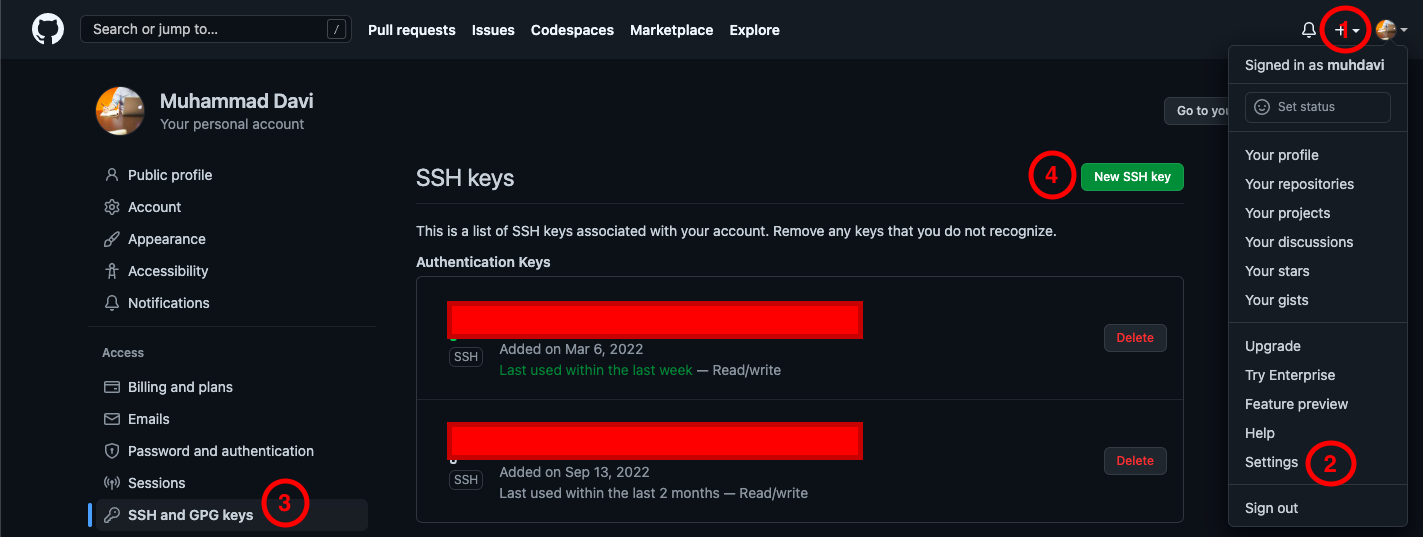
\includegraphics[width=.9\textwidth]{github-1}
\caption{Lankah-langkah Menambah SSH-Key di GitHub}
\label{gam:langkah-ssh}
\end{figure}

Kode SSH-Key yang telah di-\textit{copy} pada langkah sebelumnya \textit{paste}-kan kode tersebut pada isian \textbf{Key} dan beri judul SSH-Key pada isian \textbf{Title}. Setelah semua diisi klik tombol \textbf{Add SSH key} untuk menyimpan SSH-Key baru tersebut.

\begin{figure}[!ht]
\centering
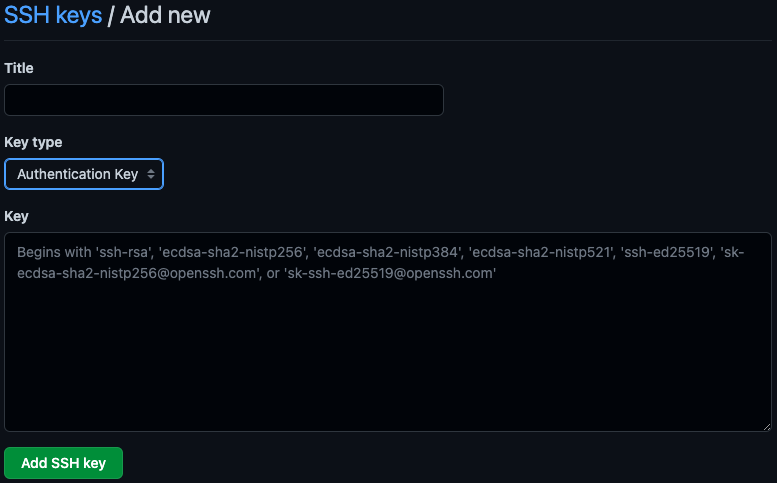
\includegraphics[width=.9\textwidth]{github-2}
\caption{Form Penambahan SSH-Key di GitHub}
\label{gam:tambah-ssh}
\end{figure}

Penjelasan lebih lanjut tentang GIT dapat membaca catatan pada link berikut \url{https://muhdavi.github.io/learn-git/}.
\end{enumerate}

\vspace*{-.5cm}
\hrulefill

%%%%%%%%%%%%%%%%%%%%%%%%%%%%%%%%%%%%%%%%%%%%%%%%%%%%%%%%
\clearpage
\newday{Part \#2}
\newthought{Instalasi Apache Hadoop}

Pada pertemuan kedua ini kegiatan yang dilakukan adalah menginstall Apache Hadoop pada \textit{environment} yang telah dibuat pada pertemuan sebelumnya. Untuk menginstall Apache Hadoop dapat mengikut langkah-langkah berikut ini:

\begin{enumerate}
\item Membuat Group dan User Baru
\begin{itemize}
\item Membuat group
\begin{lstlisting}[language=Terminal]
 sudo addgroup hadoop
\end{lstlisting}

\item Membuat User Baru dan Menambahkan ke Group
\begin{lstlisting}[language=Terminal]
 sudo adduser -ingroup hadoop hdfs
\end{lstlisting}

\item Ubah Hak Akses
\begin{lstlisting}[language=Terminal]
 sudo visudo
\end{lstlisting}

\item Tambahkan Kode
\begin{lstlisting}
 hdfs	ALL=(ALL:ALL) ALL
\end{lstlisting}

\item Ganti ke User Baru
\begin{lstlisting}[language=Terminal]
 su - hdfs
\end{lstlisting}
\end{itemize}

\item Install Java
\begin{lstlisting}[language=Terminal]
 sudo apt update
 sudo apt install openjdk-8-jdk -y
\end{lstlisting}


\item Verifikasi Hasil Instalasi Java
\begin{lstlisting}[language=Terminal]
 java -version
\end{lstlisting}

Jika instalasi java berhasil tanpa ada bug atau error maka akan menampilkan hasil seperti pada Gambar \ref{gam:java-version}.

\begin{figure}
\setlength{\belowcaptionskip}{-10pt}
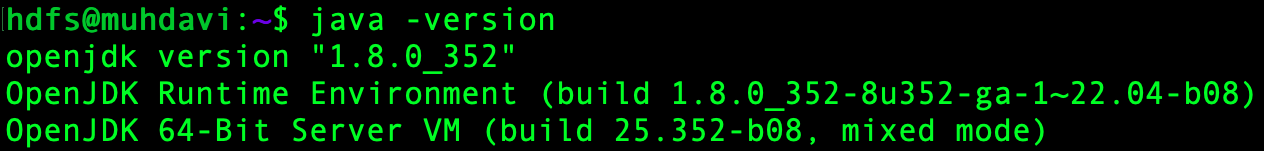
\includegraphics[width=\textwidth]{java-version}
\caption{Versi Java yang Terinstall}
\label{gam:java-version}
\end{figure}

\item Setting SSH
\begin{itemize}
\item Uninstall OpenSSH
\begin{lstlisting}[language=Terminal]
 sudo apt remove openssh-server openssh-client
\end{lstlisting}

\item Install OpenSSH Baru
\begin{lstlisting}[language=Terminal]
 sudo apt update
 sudo apt install openssh-server openssh-client
 sudo ufw allow 22
 sudo systemctl restart ssh
 sudo apt install ssh
 sudo apt install rsync
\end{lstlisting}

\item Generate Key
\begin{lstlisting}[language=Terminal]
 ssh-keygen -t dsa -P '' -f /home/hdfs/.ssh/id_dsa
 cat /home/hdfs/.ssh/id_dsa.pub >> /home/hdfs/.ssh/authorized_keys
 ssh-keygen -t rsa
\end{lstlisting}

\item Coba Masuk via SSH
\begin{lstlisting}[language=Terminal]
 ssh localhost
\end{lstlisting}

\item Jika masih harus memasukkan password, lanjutkan langakh berikut.
\begin{lstlisting}[language=Terminal]
 ssh-keygen -t rsa
 cat /home/hdfs/.ssh/id_rsa.pub >> /home/hdfs/.ssh/authorized_keys
 chmod og-wx /home/hdfs/.ssh/authorized_keys
 sudo apt update
\end{lstlisting}

\item Coba Masuk via SSH Lagi
\begin{lstlisting}[language=Terminal]
 ssh localhost
\end{lstlisting}

\item Jika sudah berhasil, keluar dengan perintah {\tt exit}
\begin{lstlisting}[language=Terminal]
 exit
\end{lstlisting}
\end{itemize}

\item Download Apache Hadoop
\begin{lstlisting}[language=Terminal]
 wget https://dlcdn.apache.org/hadoop/common/hadoop-3.3.5/hadoop-3.3.5.tar.gz
\end{lstlisting}

\item Ekstrak Apache Hadoop
\begin{lstlisting}[language=Terminal]
 tar -xzvf hadoop-3.3.4.tar.gz 
\end{lstlisting}

\begin{itemize}
\item x $\Rightarrow$ ekstrak file arsip.
\item z $\Rightarrow$ filter file arsip melalui gzip.
\item v $\Rightarrow$ menampilkan proses.
\item f $\Rightarrow$ nama file arsip.
\end{itemize}

\item Pindahkan hasil ekstraksi ke {\tt /usr/local/}
\begin{lstlisting}[language=Terminal]
 sudo mv hadoop-3.3.4 /usr/local/hadoop
\end{lstlisting}

\item Ubah Hak Akses {\tt /usr/local/hadoop}
\begin{lstlisting}[language=Terminal]
 sudo chown -R hdfs:hadoop /usr/local/hadoop
 sudo chmod -R 777 /usr/local/hadoop
\end{lstlisting}

\item Edit file {\tt sysctl.conf} untuk Disable IPV6
\begin{itemize}
\item Buka file {\tt sysctl.conf}
\begin{lstlisting}[language=Terminal]
 sudo nano /etc/sysctl.conf
\end{lstlisting}

\item Tambahkan Kode
\begin{lstlisting}[language=Bash]
net.ipv6.conf.all.disable_ipv6=1
net.ipv6.conf.lo.disable_ipv6=1
net.ipv6.conf.default_ipv6=1
\end{lstlisting}
\end{itemize}

\item Edit file {\tt hadoop-env.sh}
\begin{lstlisting}[language=Terminal]
 cd /usr/local/hadoop/etc/hadoop
 sudo nano hadoop-env.sh
\end{lstlisting}

\begin{lstlisting}[language=Bash]
export JAVA_HOME=/usr/lib/jvm/java-8-openjdk-amd64
export HADOOP_OPTS=-Djava.net.preferIPv4Stack=true
export HADOOP_HOME_WARN_SUPPRESS="TRUE"
export HADOOP_ROOT_LOGGER="WARN"
\end{lstlisting}

\item Menambahkan Hadoop ke {\tt .bashrc}
\begin{lstlisting}[language=Terminal]
 sudo nano /home/hdfs/.bashrc
\end{lstlisting}

\begin{lstlisting}[language=Bash]
# Hadoop Location
export HADOOP_HOME=/usr/local/hadoop
export HADOOP_CONF_DIR=/usr/local/hadoop/etc/hadoop
export HADOOP_MAPRED_HOME=/usr/local/hadoop
export HADOOP_COMMON_HOME=/usr/local/hadoop
export HADOOP_HDFS_HOME=/usr/local/hadoop
export YARN_HOME=/usr/local/hadoop
export PATH=$PATH:/usr/local/hadoop/bin
export PATH=$PATH:/usr/local/hadoop/sbin

# Hadoop Native Location
export HADOOP_COMMON_LIB_NATIVE_DIR=$HADOOP_HOME/lib/native
export HADOOP_OPTS="$HADOOP_OPTS -Djava.library.path=$HADOOP_HOME/lib/native"
export LD_LIBRARY_PATH=$HADOOP_HOME/lib/native
\end{lstlisting}

\begin{lstlisting}[language=Terminal]
 source /home/hdfs/.bashrc
\end{lstlisting}

\item Verifikasi Hasil Instalasi Hadoop
\begin{lstlisting}[language=Terminal]
 hadoop version
\end{lstlisting}

Jika instalasi hadoop berhasil, maka ketika mengecek versi hadoop akan muncul seperti yang diperlihatkan pada Gambar \ref{gam:hadoop-version}.
\begin{figure}[!ht]
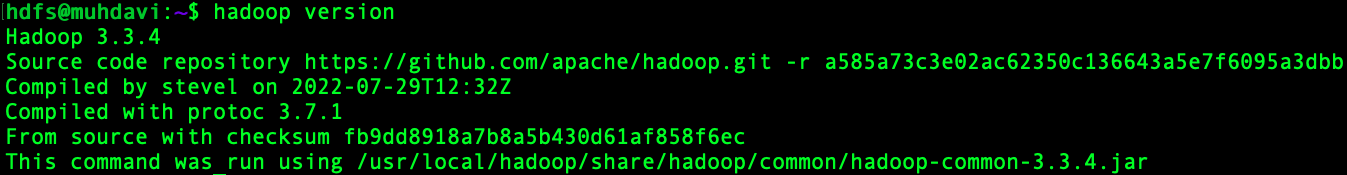
\includegraphics[width=\textwidth]{hadoop-version}
\caption{Versi Hadoop Terinstall 3.3.4}
\label{gam:hadoop-version}
\end{figure}
\end{enumerate}
 
\hrulefill

%%%%%%%%%%%%%%%%%%%%%%%%%%%%%%%%%%%%%%%%%%%%%%%%%%%%%%%%
\clearpage
\newthought{Konfigurasi Apache Hadoop}

Setelah selesai meng-install Hadoop, kita perlu konfigurasi beberapa file Hadoop agar memudahkan kita dalam memonitoring ekosistem Hadoop yang telah diinstall.

\begin{enumerate}
\item Konfigurasi File Hadoop \\
Beberapa file Hadoop yang perlu dikonfigurasi berada pada folder {\tt hadoop/etc/hadoop} seperti yang diperlihatkan pada Gambar \ref{gam:file-hadoop}. Konfigurasi file-file tersebut dapat menggunakan {\tt nano} diikuti nama file. Sisipkan kode konfigurasi diantara tag {\tt <configuration> $\cdots$ </configuration>}.

\begin{figure}[!ht]
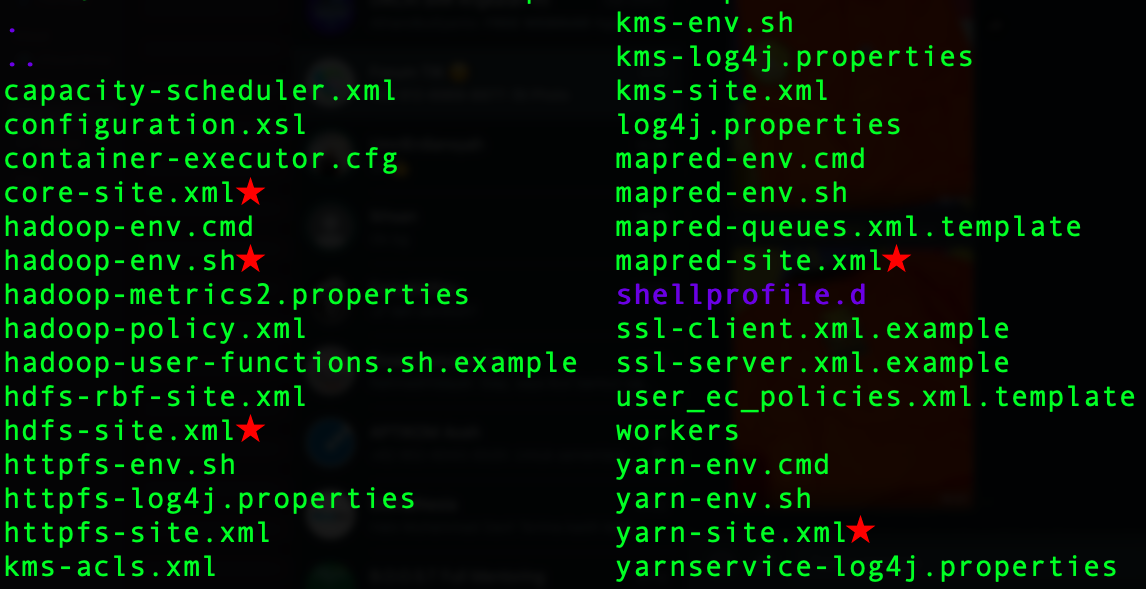
\includegraphics[width=\textwidth]{file-hadoop}
\caption{File Konfigurasi Hadoop}
\label{gam:file-hadoop}
\end{figure}

Berikut bebrapa file yang perlu dikonfigurasi dan lakukan dengan hati-hati serta teliti malalui perintah berikut:
\begin{lstlisting}[language=Terminal]
 cd /usr/local/hadoop/etc/hadoop
 sudo nano nama-file
\end{lstlisting}

\begin{itemize}

\item {\tt sudo nano core-site.xml}
\begin{lstlisting}[language=XML]
<property>
	<name>hadoop.tmp.dir</name>
	<value>/app/hadoop/tmp</value>
</property>
<property>
	<name>fs.default.name</name>
	<value>hdfs://localhost:9000</value>
</property>
\end{lstlisting}

\item {\tt sudo nano hdfs-site.xml}
\begin{lstlisting}[language=XML]
<property>
	<name>dfs.replication</name>
	<value>1</value>
</property>
<property>
	<name>dfs.namenode.name.dir</name>
	<value>file:/usr/local/hadoop/yarn_data/hdfs/namenode</value>
</property>
<property>
	<name>dfs.datanode.data.dir</name>
	<value>file:/usr/local/hadoop/yarn_data/hdfs/datanode</value>
</property>
\end{lstlisting}

\item {\tt sudo nano mapred-site.xml}
\begin{lstlisting}[language=XML]
<property>
	<name>mapred.framework.name</name>
	<value>yarn</value>
</property>
<property>
	<name>mapreduce.jobhistory.address</name>
	<value>localhost:10020</value>
</property>
\end{lstlisting}

\item {\tt sudo nano yarn-site.xml}
\begin{lstlisting}[language=XML]
<property>
	<name>yarn.nodemanager.aux-services</name>
	<value>mapreduce_shuffle</value>
</property>
<property>
	<name>yarn.nodemanager.aux-services.mapreduce.shuffle.class</name>
	<value>org.apache.hadoop.mapred.ShuffleHandler</value>
</property>
\end{lstlisting}
\end{itemize}

\item Membuat Folder Sementara (\textit{Temporary}) untuk HDFS
\begin{lstlisting}[language=Terminal]
 sudo mkdir -p /app/hadoop/tmp
 sudo chmod -R 777 /app/hadoop/tmp
 sudo chown -R hdfs:hadoop /app/hadoop/tmp
\end{lstlisting}

\item Membuat Folder {\tt namenode} dan {\tt datanode}
\begin{lstlisting}[language=Terminal]
 sudo mkdir -p /usr/local/hadoop/yarn_data/hdfs/namenode
 sudo mkdir -p /usr/local/hadoop/yarn_data/hdfs/datanode
 sudo chown -R hdfs:hadoop /usr/local/hadoop/yarn_data/hdfs/namenode
 sudo chown -R hdfs:hadoop /usr/local/hadoop/yarn_data/hdfs/datanode
 sudo chmod -R 777 /usr/local/hadoop/yarn_data/hdfs/namenode
 sudo chmod -R 777 /usr/local/hadoop/yarn_data/hdfs/datanode
\end{lstlisting}

\item Jalankan Perintah Format HDFS
\begin{lstlisting}[language=Terminal]
 hdfs namenode -format
\end{lstlisting}

\item Jalankan Hadoop Service
\begin{lstlisting}[language=Terminal]
 start-dfs.sh
 start-yarn.sh
\end{lstlisting}

\clearpage
\item Cek Hadoop Service
\begin{itemize}
\item Jalankan perintah {\tt jps}
\item Akses melalui web browser dengan alamat \url{http://localhost:9870}\footnote{Seperti yang diperlihatkan pada Gambar \ref{gam:namenode}} atau \url{http://localhost:8088}\footnote{Seperti yang diperlihatkan pada Gambar \ref{gam:resourcemanager}}.
\end{itemize}

\begin{figure}[!ht]
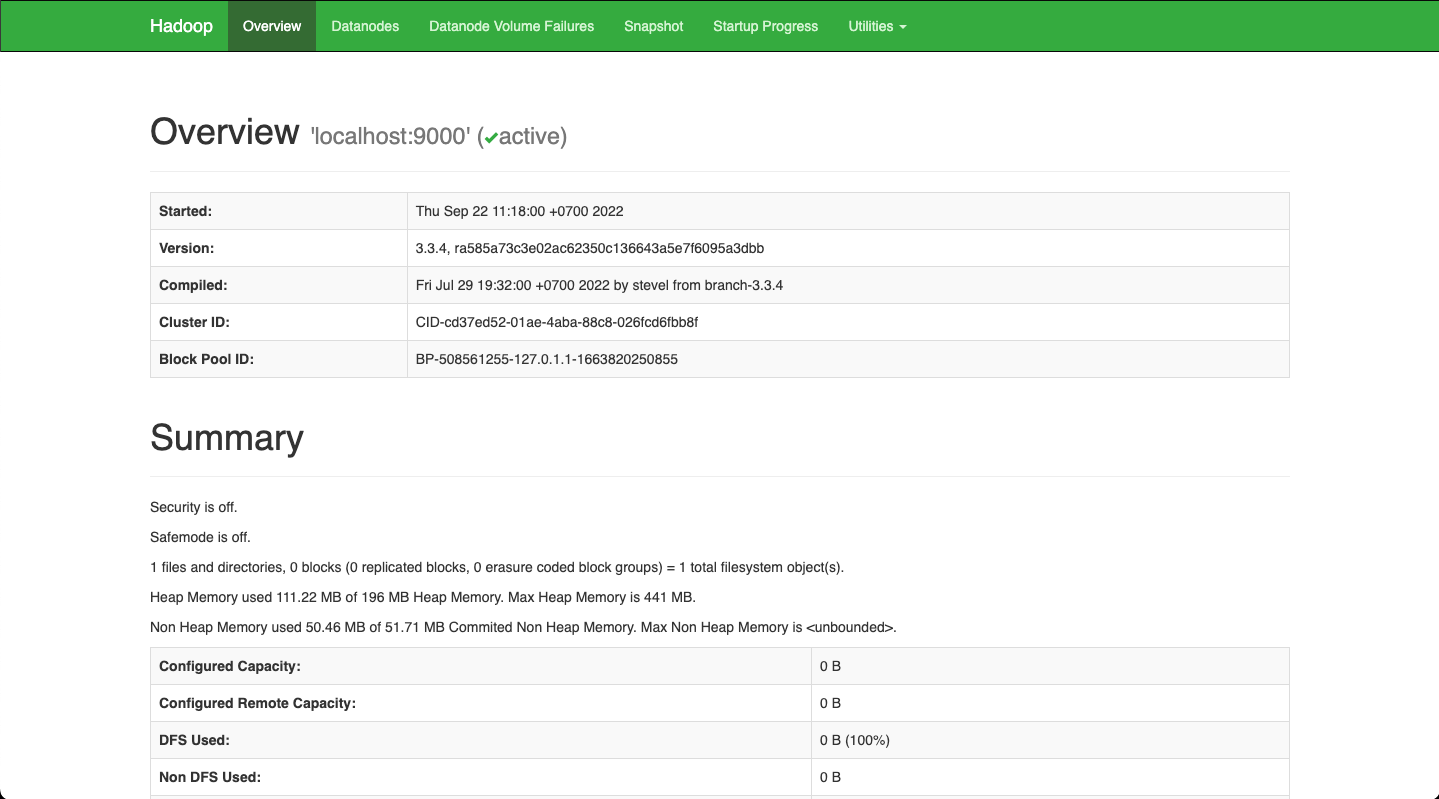
\includegraphics[width=\textwidth]{namenode}
\label{gam:namenode}
\end{figure}
\vspace*{-.7cm}
\begin{figure}[!ht]
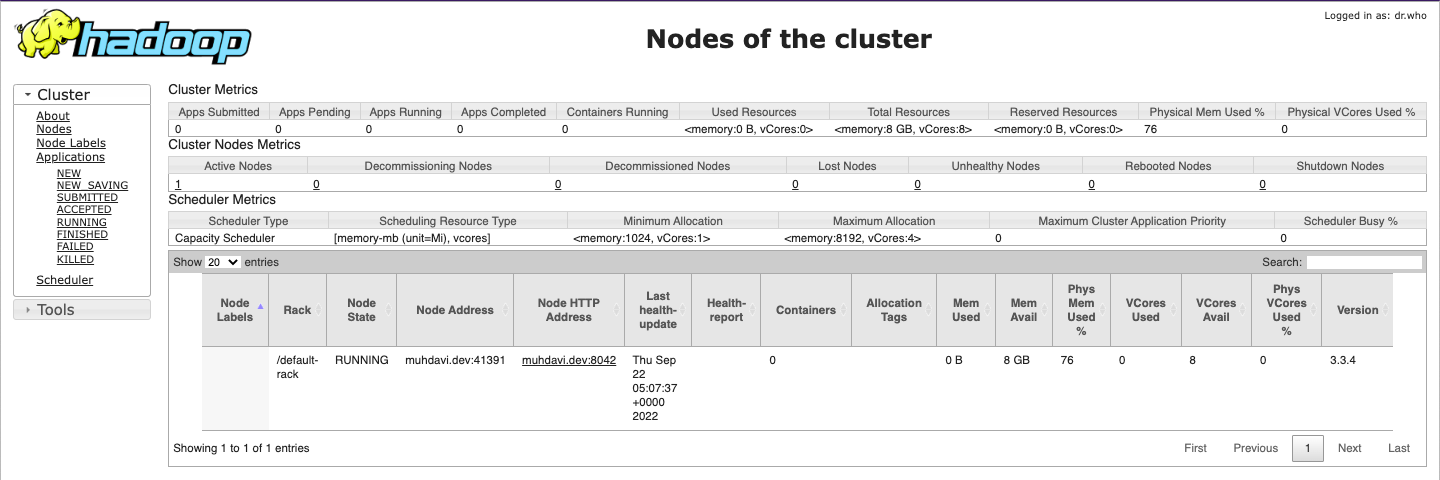
\includegraphics[width=\textwidth]{resourcemanager}
\caption{Resource Manager Hadoop}
\label{gam:resourcemanager}
\end{figure}

\vspace*{-.7cm}
\item Hentikan Hadoop Service
\begin{itemize}
\item Hentikan Service Tertentu
\begin{lstlisting}[language=Terminal]
 stop-dfs.sh
\end{lstlisting} 
atau
\begin{lstlisting}[language=Terminal]
 stop-yarn.sh
\end{lstlisting}
 
\item Hentikan Semua Service
\begin{lstlisting}[language=Terminal]
 stop-all.sh
\end{lstlisting}
\end{itemize}
\end{enumerate}
% mounting data shared folder
% sudo mount -t vboxsf share /mnt/share

\vspace*{.1cm}

\newday{HK \#1}

\hrulefill

%%%%%%%%%%%%%%%%%%%%%%%%%%%%%%%%%%%%%%%%%%%%%%%%%%%%%%%%
\clearpage
\newday{Part \#3}
\newthought{Program WordCount bawaan Hadoop}

Jika sudah selesai malakukan instalasi Hadoop, maka dapat mencoba program bawaan Hadoop untuk memahami bagaimana proses dan cara kerja Hadoop dalam memproses data input hingga menghasilkan sebuah output. Salah satu program yang sudah disediakan oleh Hadoop adalah WordCount, yaitu program menghitung jumlah kata dalam data input yang diberikan. Silahkan ikuti langkah-langkah berikut ini untuk mengetahui cara penggunaan program WordCount.

\begin{enumerate}
\item Jalankan Hadoop Service
\begin{lstlisting}[language=Terminal]
 start-dfs.sh
 start-yarn.sh
\end{lstlisting}

\item Buat folder input di HDFS
\begin{lstlisting}[language=Terminal]
 hadoop fs -mkdir /input
\end{lstlisting}

\item Download data teks dengan perintah \textit{wget}
\begin{lstlisting}[language=Terminal]
 wget "https://raw.githubusercontent.com/muhdavi-pnl/NET17237/main/data/4300.txt"
\end{lstlisting}

\item Pindahkan file {\tt 4300.txt} ke folder input di HDFS
\begin{lstlisting}[language=Terminal]
 hadoop fs -put 4300.txt /input
\end{lstlisting}

\item Jalankan program WordCount
\begin{lstlisting}[language=Terminal]
 hadoop jar /usr/local/hadoop/share/hadoop/mapreduce/hadoop-mapreduce-examples-3.3.4.jar wordcount /input/4300.txt /output
\end{lstlisting} 
%hadoop jar /usr/local/hadoop/share/hadoop/mapreduce/hadoop-mapreduce-examples-3.2.0.jar wordcount /input/ /output2 -> untuk semua file dari folder input

\item Cek Hasil
\begin{lstlisting}[language=Terminal]
 hadoop fs -ls /output
\end{lstlisting} 

\item Lihat Hasil
\begin{lstlisting}[language=Terminal]
 hadoop fs -cat /output/part-r-00000
\end{lstlisting} 
\end{enumerate}

\newthought{Tugas Praktikum} \\
\begin{enumerate}
%\item Buatlah sebuah konfigurasi environment Big Data dengan beberapa Node sesuai dengan jumlah anggota dalam kelompok.
%\item Jalankan program \textit{WordCount} dengan data yang telah didownload sebelumnya, yaitu: \textbf{4300.txt}.
\item Buatlah Laporan tentang perintah-perintah pada Hadoop dalam format PDF sesuai template yang diberikan di GitHub Classroom. 
\item Format penamaan file PDF adalah \textit{NIM - Nama Mahasiswa.pdf}.
\end{enumerate}

\hrulefill

%%%%%%%%%%%%%%%%%%%%%%%%%%%%%%%%%%%%%%%%%%%%%%%%%%%%%%%%
\clearpage
\newday{Part \#4}
\newthought{Program WordCount dengan Java}

Pada pertemuan sebelumnya telah mencoba program WordCount bawaan Hadoop. Jika dengan program bawaan Hadoop sudah dapat mendapatkan hasil, artinya Hadoop kita sudah bisa digunakan untuk menjalankan program. Ikuti beberapa langkah berikut untuk memberikan pemahaman bagaimana proses membuat program, menyiapkan data, meng-compile program hingga menjalankan program dan memperoleh hasilnya.

\begin{enumerate}
\item Pastikan Hadoop Service sudah berjalan
\item Pastikan data input pada pertemuan sebelumnya masih tersedia di HDFS
\begin{lstlisting}[language=Terminal]
 hadoop fs -ls /input
\end{lstlisting}

\item Buat file baru dengan nama dan kode berikut
\begin{lstlisting}[language=Terminal]
 sudo nano WordCount.java
\end{lstlisting} 
\lstinputlisting[caption=Code WordCount Java, label={lst:wordcount-java}, language=Java]{code/wordcount-java.java}
% https://github.com/muhdavi/kode-practice-big-data/blob/main/WordCountJava/src/main/java/WordCount.java

\item Buat classpath
\begin{lstlisting}[language=Terminal]
 export HADOOP_CLASSPATH=$($HADOOP_HOME/bin/hadoop classpath)
\end{lstlisting} 

\item Buat folder baru untuk menampung hasil \textit{compile} program java dan ubah hak aksesnya
\begin{lstlisting}[language=Terminal]
 sudo mkdir JavaCompiled
 sudo chmod -R 777 JavaCompiled
\end{lstlisting}

\item Compile file WordCount.java
\begin{lstlisting}[language=Terminal]
 javac -classpath $HADOOP_CLASSPATH -d JavaCompiled WordCount.java
\end{lstlisting}

\item Mengubah file menjadi executable .jar
\begin{lstlisting}[language=Terminal]
 jar -cvf WordCount.jar -C JavaCompiled/ .
\end{lstlisting}

\item Jalankan program WordCount
\begin{lstlisting}[language=Terminal]
 hadoop jar WordCount.jar WordCount /input/4300.txt /ResultWordCountJava
\end{lstlisting}

\item Cek Hasil
\begin{lstlisting}[language=Terminal]
 hadoop fs -ls /ResultWordCountJava
\end{lstlisting}

\item Lihat Hasil
\begin{lstlisting}[language=Terminal]
 hadoop fs -cat /ResultWordCountJava/part-r-00000
\end{lstlisting} 
\end{enumerate}

\newday{HK \#2}

\hrulefill

%%%%%%%%%%%%%%%%%%%%%%%%%%%%%%%%%%%%%%%%%%%%%%%%%%%%%%%%
\clearpage
\newday{Part \#5}
\newthought{Program WordCount dengan Python}

\begin{enumerate}
\item Pastikan Hadoop Service dan Spark Service berjalan
\item Pastikan data input pada pertemuan sebelumnya masih tersedia di HDFS
\item Buat folder baru untuk menyimpan file Python
\begin{lstlisting}[language=Terminal]
 sudo mkdir WordCountPython
\end{lstlisting}

\item Buat file baru dengan nama dan kode berikut
\begin{itemize}
\item {\tt map.py}
\begin{lstlisting}[language=Terminal]
 sudo nano WordCountPython/map.py
\end{lstlisting}
 
\lstinputlisting[caption=Code Map Python, label={lst:map-python}, language=Python]{code/map.py}
%{\tt wget https://raw.githubusercontent.com/muhdavi/kode-practice- big-data/main/WordCountPython/map.py}

\item {\tt reduce.py}
\begin{lstlisting}[language=Terminal]
 sudo nano WordCountPython/reduce.py
\end{lstlisting} 
\lstinputlisting[caption=Code Reduce Python, label={lst:reduce-python}, language=Python]{code/reduce.py}
%{\tt wget https://raw.githubusercontent.com/muhdavi/kode-practice- big-data/main/WordCountPython/reduce.py}
\end{itemize}

\item Ubah Hak Akses
\begin{lstlisting}[language=Terminal]
 sudo chmod +x -R WordCountPython/
\end{lstlisting}

%\item Mencoba Program di Local
%\begin{lstlisting}[language=Terminal]
% echo jangan heran jika orang cantik merasa jelek sementara orang yang jelek merasa cantik | WordCountPython/map.py | sort | WordCountPython/reduce.py
%\end{lstlisting}

\item Jalankan Program menggunakan Hadoop
\begin{lstlisting}[language=Terminal]
 hadoop jar /usr/local/hadoop/share/hadoop/tools/lib/hadoop-streaming-3
 .3.4.jar -mapper /home/hdfs/WordCountPython/map.py -reducer /home/hdfs
 /WordCountPython/reduce.py -input /input/4300.txt -output /Re
 sultWordCountPython
\end{lstlisting}

\item Cek Hasil
\begin{lstlisting}[language=Terminal]
 hadoop fs -ls /ResultWordCountPython
\end{lstlisting}

\item Lihat Hasil 
\begin{lstlisting}[language=Terminal]
 hadoop fs -cat /ResultWordCountPython/part-00000
\end{lstlisting}

\end{enumerate}

\hrulefill

%%%%%%%%%%%%%%%%%%%%%%%%%%%%%%%%%%%%%%%%%%%%%%%%%%%%%%%%
\clearpage
\newday{Part \#6}
\newthought{Instalasi Apache Spark (PySpark)}

\begin{enumerate}
\item Download Apache Spark
\begin{lstlisting}[language=Terminal]
 wget https://dlcdn.apache.org/spark/spark-3.3.3/spark-3.3.3-bin-hadoop3.tgz
\end{lstlisting}

\item Ekstrak Apache Spark
\begin{lstlisting}[language=Terminal]
 tar -xzvf spark-3.3.1-bin-hadoop3.tgz
\end{lstlisting}

\item Pindahkan hasil ekstraksi ke {\tt /usr/local/}
\begin{lstlisting}[language=Terminal]
 sudo mv spark-3.3.1-bin-hadoop3 /usr/local/spark
\end{lstlisting} 

\item Menambahkan Spark ke {\tt .bashrc}
\begin{lstlisting}[language=Terminal]
 sudo nano /home/hdfs/.bashrc
\end{lstlisting} 
\begin{lstlisting}[language=Bash, label={lst:bash-spark}, caption=Code Konfig Apaceh Spark]
# Spark Location
export SPARK_HOME=/usr/local/spark
export PATH=$PATH:$SPARK_HOME/bin:$SPARK_HOME/sbin
\end{lstlisting}
\begin{lstlisting}[language=Terminal]
 source /home/hdfs/.bashrc
\end{lstlisting}

\item Verifikasi Hasil Instalasi Spark
\begin{lstlisting}[language=Terminal]
 pyspark ---version
\end{lstlisting}

\begin{figure}[!ht]
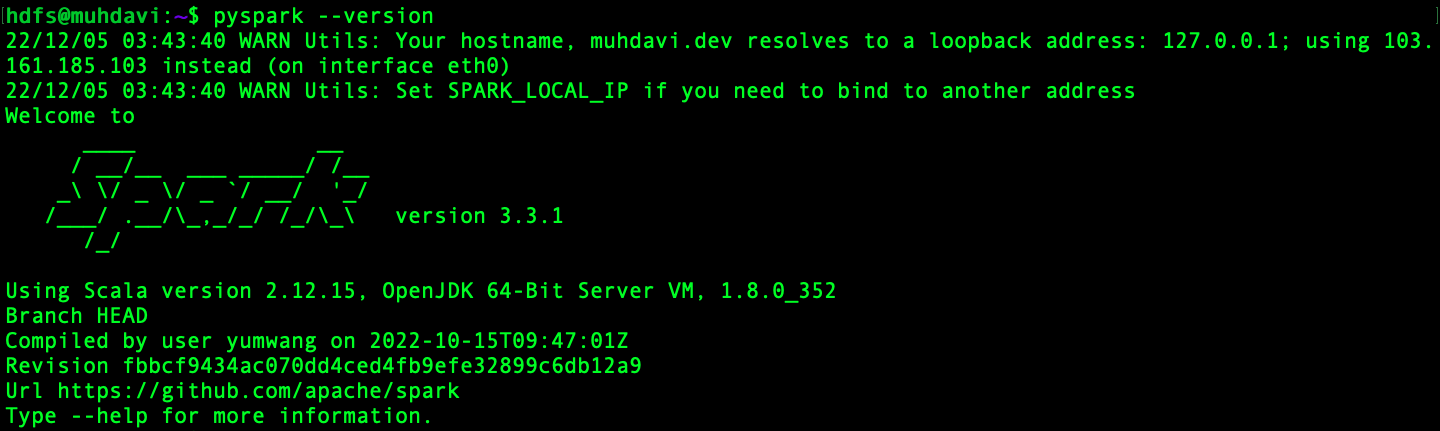
\includegraphics[width=\textwidth]{spark-version}
\caption{Versi Spark Terinstall 3.3.1 }
\label{gam:form-ssh}
\end{figure}

\item Jalankan Spark Service
\begin{lstlisting}[language=Terminal]
 start-master.sh
\end{lstlisting}

\item Hentikan Spark Service
\begin{lstlisting}[language=Terminal]
 stop-master.sh
\end{lstlisting} 
\end{enumerate}

\hrulefill

%%%%%%%%%%%%%%%%%%%%%%%%%%%%%%%%%%%%%%%%%%%%%%%%%%%%%%%%
\clearpage
\newday{Part \#7}
\newthought{Program WordCount dengan PySpark}

\begin{enumerate}
\item Pastikan Hadoop Service dan Spark Service berjalan
\item Pastikan data input pada pertemuan sebelumnya masih tersedia di HDFS
\item Buat folder baru untuk menyimpan file Python
\begin{lstlisting}[language=Terminal]
 sudo mkdir WordCountPySpark
 cd WordCountPySpark
\end{lstlisting}

\item Buat file baru dengan nama dan kode berikut
\begin{lstlisting}[language=Terminal]
 sudo nano WordCount.py
\end{lstlisting} 
\lstinputlisting[caption=Code WordCount PySpark, label={lst:wordcount-pyspark}, language=Python]{code/wordcount-pyspark.py}

\item Jalankan Program menggunakan PySpark
\begin{lstlisting}[language=Terminal]
 spark-submit WordCount.py
\end{lstlisting}

\item Cek Hasil
\begin{lstlisting}[language=Terminal]
 hadoop fs -ls /ResultWordCountPySpark
\end{lstlisting}

\item Lihat Hasil
\begin{lstlisting}[language=Terminal]
 hadoop fs -cat /ResultWordCountPySpark/part-00000
\end{lstlisting} 
\end{enumerate}


\hrulefill

%%%%%%%%%%%%%%%%%%%%%%%%%%%%%%%%%%%%%%%%%%%%%%%%%%%%%%%%
\clearpage
%\newday{\#15 - Tugas Individu menggantikan 15 Desember 2022}

\newthought{Program Machine Learning dengan PySpark}

Setelah mencoba beberapa kali program WordCount baik menggunakan bahasa pemograman Java maupun Python. Sekarang coba membuat program \textit{machine learning} menggunakan Python dan jalankan menggunakan PySpark dengan \textit{spark-submit}. Ikutilah langkah-langkah berikut ini secara cermat dan teliti.

\begin{enumerate}
\item Pastikan Hadoop dan Spark berjalan
\item Pastikan package sudah tersedia
\begin{lstlisting}[language=Terminal]
 pip list
\end{lstlisting} 
\begin{multicols}{3}
\begin{itemize}
\item pandas
\item matplotlib
\item numpy
\item seaborn
\item scikit-learn
\end{itemize}
\end{multicols}

Jika package tersebut belum tersedia, install terlebih dahulu menggunakan {\tt pip}, misalnya {\tt pip install scikit-learn}.

\item Buat file baru dengan nama dan kode berikut
\begin{lstlisting}[language=Terminal]
 sudo nano MLPySpark.py
\end{lstlisting} 
\lstinputlisting[caption=Code Machine Learning PySpark, label={lst:ml-pyspark}, language=Python]{code/ml-pyspark.py}

\item Jalankan Program menggunakan PySpark
\begin{lstlisting}[language=Terminal]
 spark-submit MLPySpark.py
\end{lstlisting}

\end{enumerate}

\newday{HK \#3}

\hrulefill

%%%%%%%%%%%%%%%%%%%%%%%%%%%%%%%%%%%%%%%%%%%%%%%%%%%%%%%%
\clearpage
%\newday{\#16 - Tugas Kelompok menggantikan 22 Desember 2022}

\newthought{Tugas Kelompok menggunakan PySpark}

\hrulefill

\begin{center}
\noindent
\textbf{\textcolor{red}{Ingat!\\ Seminar tanggal 20/22 Desember 2023.}}
\end{center}

\hrulefill

%%%%%%%%%%%%%%%%%%%%%%%%%%%%%%%%%%%%%%%%%%%%%%%%%%%%%%%%

\clearpage
\bibliographystyle{plain}
\bibliography{lab_notes}

\end{document}

%%%%%%%%%%%%%%%%%%%%%%%%%%%%%%%%%%%%%%%%%%%%%%%%%%%%%%%%
